\documentclass[11pt]{article}
\usepackage{setspace}
\usepackage[a4paper,margin=1in]{geometry}
\geometry{margin=0.85in}
\setstretch{1.0}
\usepackage{graphicx}
\usepackage{array}
\usepackage{setspace}
\usepackage{parskip}
\usepackage{ragged2e}

\pagestyle{empty}
\setstretch{1.05}

\begin{document}


% Title
\begin{center}
    {\Large \textbf{Job Application}} \\[3cm]
    
    {\Huge \textbf{Zhongli Wang}} \\[0.4cm]
    
    {\huge Application for Quantitative Researcher}
\end{center}

\vspace{0.6cm}

% Large picture in the middle
\begin{center}
    \IfFileExists{../zhongli-wang-profile.jpg}{
        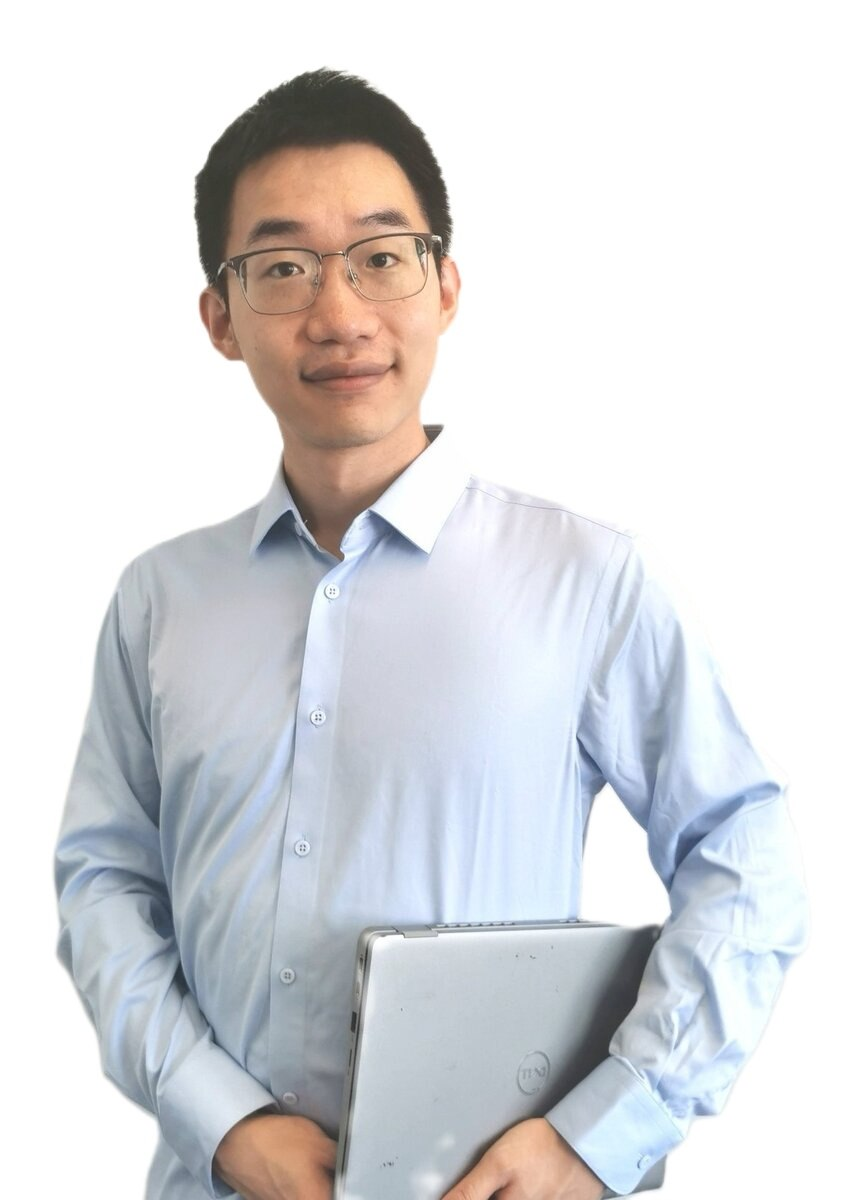
\includegraphics[
            width=0.55\textwidth,
            height=0.45\textheight,
            keepaspectratio
        ]{../zhongli-wang-profile.jpg}
    }{
        \vspace{0.45\textheight}
    }
\end{center}

\vspace{0.7cm}

% \vspace{3cm}


% Personal details
\begin{center}
\renewcommand{\arraystretch}{1.35}
\begin{tabular}{>{\bfseries}p{4.2cm} p{8.5cm}}


Address: & Astastrasse 22, 33617 Bielefeld, Germany \\

Number: & +49 160 9541 6015 \\

Email: & nkwangzhongli@gmail.com \\
\end{tabular}
\end{center}

\vfill

% \begin{center}
%     \small Last updated: \today
% \end{center}
\newpage
\enlargethispage{4\baselineskip}

\begin{flushright}
Zhongli Wang \\
Astastrasse 22 \\
33617 Bielefeld \\
Germany \\
\end{flushright}

\vspace{0.1cm}

\noindent
Frontier Asset Management \\
Hong Kong

\vspace{0.1cm}

\noindent
Application for Quantitative Researcher \\

\vspace{0.05cm}

\noindent Dear Leslie Zhang,

I am writing to apply for the Quantitative Researcher position at Frontier Asset Management in Hong Kong. 
I am completing the final stage of my Ph.D. in Economics at Bielefeld University, with my defense scheduled for September 21, 2026, 
and I also hold an M.A. in Business and Economics with a Banking and Finance major and a B.Sc. in Finance. 
My background combines statistical modeling, Python-based computational research, financial data analysis, and machine learning.

I plan to build the next stage of my career in Hong Kong, and this role is attractive because it connects rigorous quantitative research with practical investment decision-making. 
The focus on equity and futures datasets, alpha signal discovery, model construction, backtesting, and strategy optimization matches the type of structured research process I have developed in economics and finance projects.

My closest fit with the mandate is the ability to turn complex data and model output into testable evidence. 
In my doctoral work, I build computational models of strategic firm behavior, estimate parameters, and analyze how market structure changes outcomes under uncertainty. 
In a published fraud detection project, I used accounting, financial, and market indicators with XGBoost and LightGBM to identify red flags in listed companies.

I would bring the following strengths to Frontier Asset Management's quantitative research team:

\begin{itemize}
    \item \textbf{Python data analysis:} Advanced Python skills for data processing, simulation, machine learning, and reproducible empirical research.
    \item \textbf{Alpha research foundation:} Experience structuring financial and behavioral indicators into model-ready datasets and testing whether signals survive validation.
    \item \textbf{Backtesting discipline:} Training in econometrics, SMM, MCMC, agent-based modeling, robustness checks, and careful interpretation of model performance.
    \item \textbf{Structured problem solving:} Finance training, quantitative economics research, and experience communicating technical results across international teams.
\end{itemize}

Although I have not yet worked in a dedicated high- or mid-frequency trading seat, my training is aligned with the analytical core of the role: cleaning noisy datasets, designing testable factors, validating models, and improving research workflows. 
I would aim to contribute through disciplined Python research pipelines, careful robustness analysis, and clear documentation that supports investment decisions.

Thank you for your time and consideration. 
I would welcome the opportunity to discuss how my research background, financial training, and coding experience can contribute to Frontier Asset Management's Quantitative Researcher mandate in Hong Kong.

\vspace{0.05cm}
\noindent Sincerely, \\[0.08cm]
\noindent Zhongli Wang \\[-0.2cm]

\vspace{0.1cm}
\noindent
\includegraphics[width=2.7cm,keepaspectratio]{../Wang-sig.jpg}

\end{document}
